% --- Preámbulo ---
\documentclass[12pt]{article}
% Márgenes
\textheight = 24cm
\textwidth = 18cm
\topmargin = -2cm
\oddsidemargin= -1cm
%\parindent = 1cm
\setlength{\parindent}{1cm}
\setlength{\parskip}{10pt}
%\definecolor{Celeste}{RGB}{65,173,231}

% Paquetes
\usepackage{amsmath,amssymb,amsfonts,latexsym}
\usepackage[T1]{fontenc}
\usepackage[utf8]{inputenc} % Codificación para poder usar acentos
\usepackage{graphicx}

% Inicio del documento
\begin{document}
	\begin{center}
		\huge \textbf{Configurar Base de Datos}
	\end{center}
	\large \textbf{Paso 1:} Hacer click sobre el botón \textit{Agregar}
	\begin{center}
		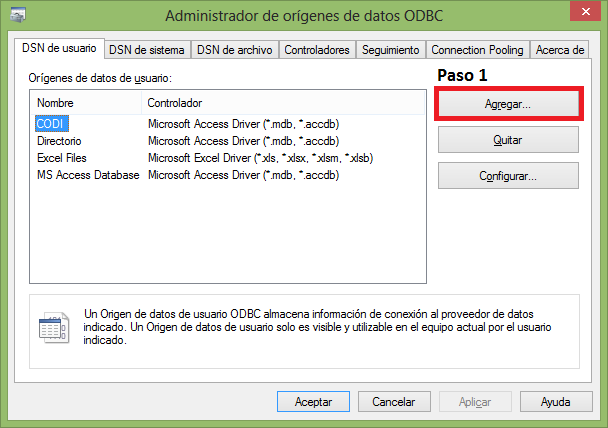
\includegraphics{Paso1}
	\end{center}
	\newpage
	\large \textbf{Paso 2 y 3:} Seleccionar el controlador \textit{Microsoft Access Driver (*.mdb, *.accdb)} y hacer click sobre el botón \textit{Finalizar}
	\begin{center}
		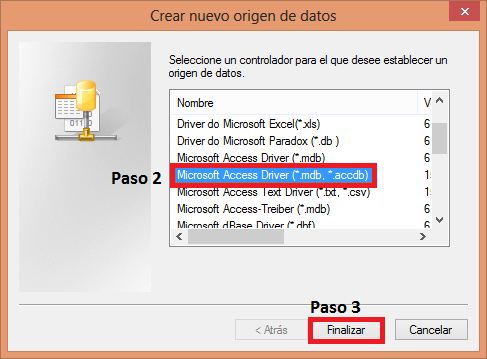
\includegraphics{Paso2y3}
	\end{center}
	\large \textbf{Paso 4:} En el campo del nombre de origen digitar \textit{CODI} y luego hacer click en el botón \textit{Seleccionar}
	\begin{center}
		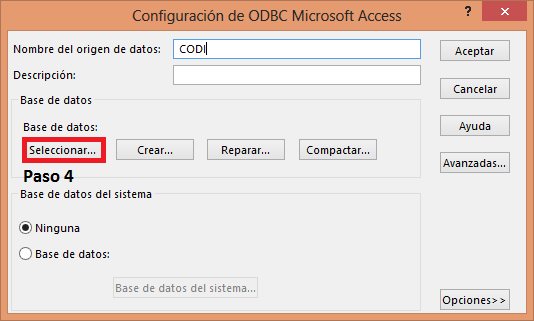
\includegraphics{Paso4}
	\end{center}
	\newpage
	\large \textbf{Paso 5:} Buscar en la carpeta de instalación de la aplicación el archivo \textit{CODI.accdb} y hacer click en el botón \textit{Aceptar}
	\begin{center}
		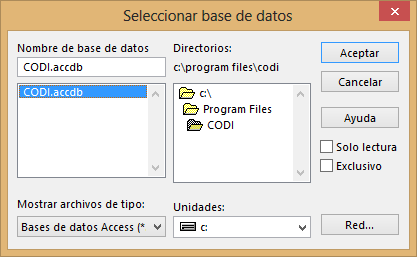
\includegraphics{Paso5}
	\end{center}
	\large \textbf{Paso 6:} Hacer click en el botón \textit{Aceptar}
	\begin{center}
		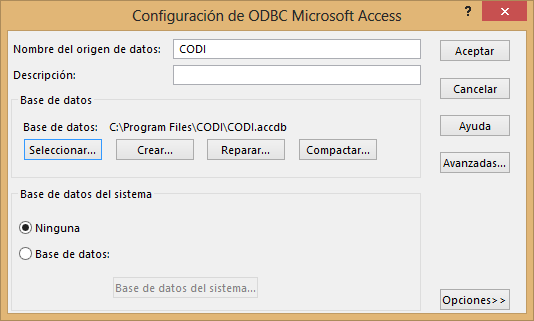
\includegraphics{Paso6}
	\end{center}
\end{document}